\chapter{Template Usage Guide}

Welcome to the Science Notes Template. This template is heavily optimized for STEM subjects like electromagnetism, signal processing, physics, and computer science. The design philosophy is centered around being compact yet readable, utilizing the classic Palatino font for a textbook-like feel.

This chapter serves as a comprehensive guide on how to utilize the various custom features bundled within this template.

\section{Highlight Boxes}
To emphasize important concepts, formulas, or examples, we've provided custom colored environments. These grab the reader's attention and help break down complex texts visually.

\begin{definition}[Eigenvector]
An eigenvector of a linear transformation is a non-zero vector that changes at most by a scalar factor when that linear transformation is applied to it.
\end{definition}

\begin{theorem}[Gauss's Law]
The net electric flux through any hypothetical closed surface is equal to $\frac{1}{\varepsilon_0}$ times the net electric charge within that closed surface:
\begin{equation}
    \Phi_E = \oint_S \mathbf{E} \cdot d\mathbf{A} = \frac{Q_{\text{enc}}}{\varepsilon_0}
\end{equation}
\end{theorem}

\begin{important}[Units and Dimensions]
Always carry your units throughout the calculation! You can easily format units using the \texttt{siunitx} package. For example, the speed of light is $c = \SI{3.00e8}{\meter\per\second}$.
\end{important}

\begin{example}
Calculate the energy of a photon with frequency $f = \SI{500}{\tera\hertz}$.
\textbf{Solution:} Using Planck's equation $E = hf$:
\[ E = (\SI{6.626e-34}{\joule\second}) \times (\SI{500e12}{\hertz}) = \SI{3.31e-19}{\joule} \]
\end{example}

\section{Displaying Code}
Writing algorithms or scripts is integral to modern science notes. We have pre-configured the \texttt{listings} package with a beautiful style to format your code nicely. 

\begin{lstlisting}[language=Python, caption={Calculating the Fibonacci sequence}]
def fibonacci(n):
    """Generate Fibonacci sequence up to n."""
    a, b = 0, 1
    sequence = []
    while a < n:
        sequence.append(a)
        a, b = b, a + b
    return sequence

print(fibonacci(100))
\end{lstlisting}

\section{Graph Plotting with PGFPlots}
Why use external tools when you can generate high-quality vector graphics directly in \LaTeX? The \texttt{pgfplots} package is incredibly powerful for 2D and 3D data visualization.

\subsection{2D Signal Graph}
\begin{figure}[H]
    \centering
    \begin{tikzpicture}
        \begin{axis}[
            width=10cm, height=5cm,
            axis lines=middle,
            xlabel={$t$ (seconds)},
            ylabel={$V(t)$ (volts)},
            grid=both,
            minor tick num=1,
            enlargelimits=true,
            samples=100,
            domain=0:4*pi
        ]
            \addplot[thick, primary] {sin(deg(x)) * exp(-0.2*x)};
            \addlegendentry{Damped Sine Wave}
        \end{axis}
    \end{tikzpicture}
    \caption{A simple 2D plot of a damped sinusoidal signal.}
\end{figure}

\subsection{3D Surface Graph}
Visualizing multivariable functions is easy with 3D plotting capabilities.

\begin{figure}[H]
    \centering
    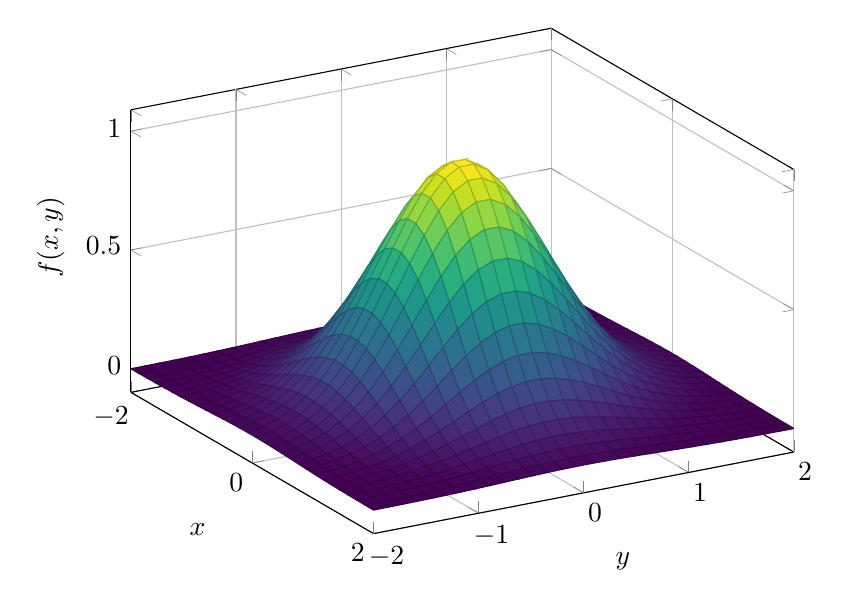
\begin{tikzpicture}
        \begin{axis}[
            view={60}{30},
            width=10cm, height=8cm,
            grid=major,
            xlabel={$x$},
            ylabel={$y$},
            zlabel={$f(x,y)$},
            colormap/viridis
        ]
            \addplot3[
                surf,
                domain=-2:2,
                domain y=-2:2,
                samples=30
            ]
            {exp(-x^2-y^2)};
        \end{axis}
    \end{tikzpicture}
    \caption{A 3D surface plot of a Gaussian function.}
\end{figure}

\section{Circuit Diagrams}
The \texttt{circuitikz} package is loaded and configured for drawing electrical circuits effortlessly.

\begin{figure}[H]
    \centering
    \begin{circuitikz}[american, scale=1.2]
        \draw (0,0) 
            to[V, l=$V_{in}$] (0,3)
            to[R, l=$R$, i=$i(t)$] (3,3)
            to[L, l=$L$] (5,3)
            to[C, l=$C$, v=$v_c(t)$] (5,0) 
            -- (0,0);
        \draw (5,3) -- (6.5,3) node[right]{$+$};
        \draw (5,0) -- (6.5,0) node[right]{$-$};
        \node at (6.5, 1.5) {$V_{out}$};
    \end{circuitikz}
    \caption{An RLC series circuit diagram drawn directly in \LaTeX.}
\end{figure}

\section{Next Steps}
Feel free to add more chapters in the \texttt{sections/} folder and include them in \texttt{main.tex} using the \verb|\input{}| command. Happy note-taking!
